\documentclass[12pt]{article}
\usepackage{fullpage,graphicx,psfrag,amsmath,amsfonts,verbatim}
\usepackage[small,bf]{caption}
\usepackage{bbm}
\input defs.tex
\usepackage{subcaption}
\usepackage{wrapfig}

\bibliographystyle{alpha}

\title{Linear Regression}
\author{Annie Marsden}

\begin{document}

\paragraph{When to impose test-data constraints for Noise-less Linear Regression}

Suppose $\exists \theta_{\textrm{true}} \in \mathbb{R}^{d}$ such that given $x \in \mathbb{R}^{d}$ we have $y_{x} = \theta_{\textrm{true}}^{T}x$. Let $\{ (x_{1}, y_{1}), \cdots, (x_{n},y_{n}) \}$ denote some set of training data and let $\{z_{1}, \cdots, z_{m} \}$ denote the test set. Suppose we know something further about the test set, namely the predictions should belong to some convex set $[a,b]$.
\begin{wrapfigure}{r}{.4\textwidth}
    \begin{minipage}{\linewidth}
    \centering\captionsetup[subfigure]{justification=centering}
    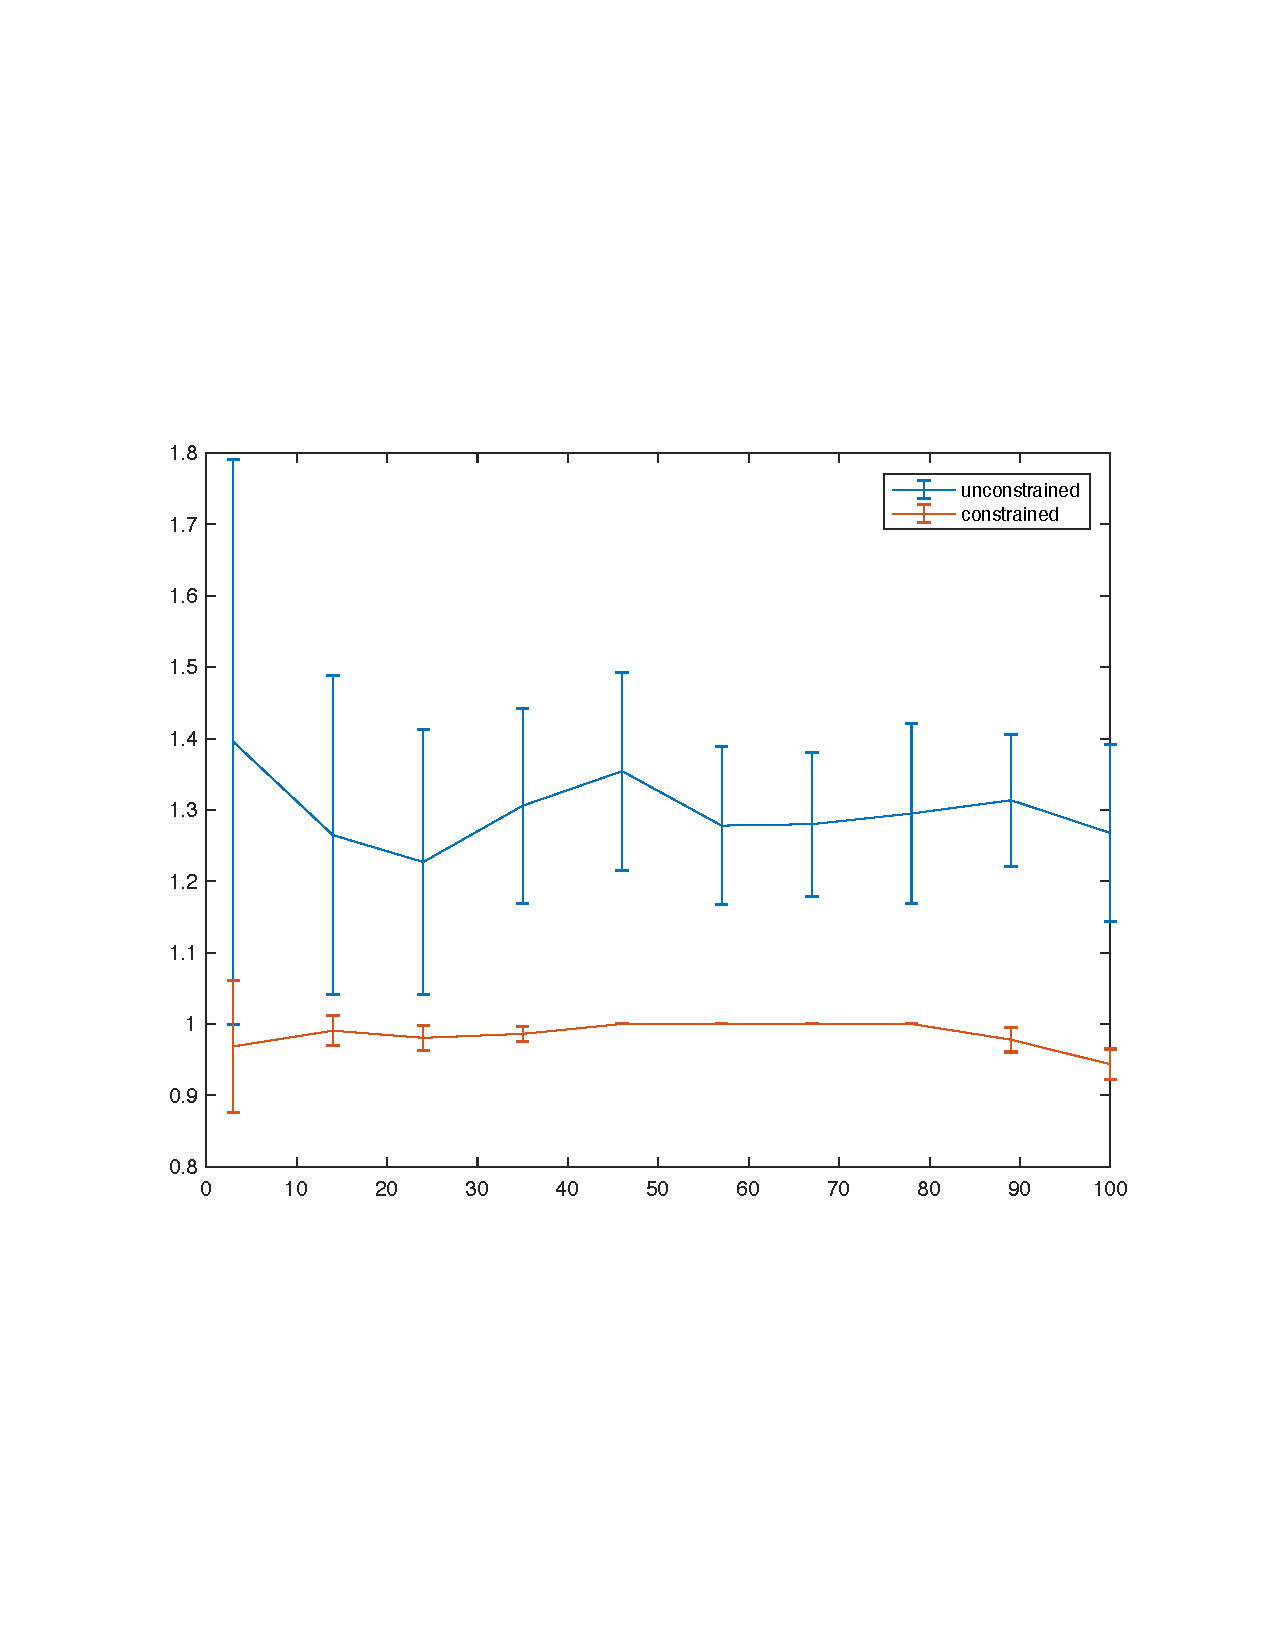
\includegraphics[width=\linewidth]{figure_7_7bound.pdf}
    \subcaption{Test data predictions are bounded to the interval $[-0.7,0.7]$}
    \label{fig:5a}\par\vfill
    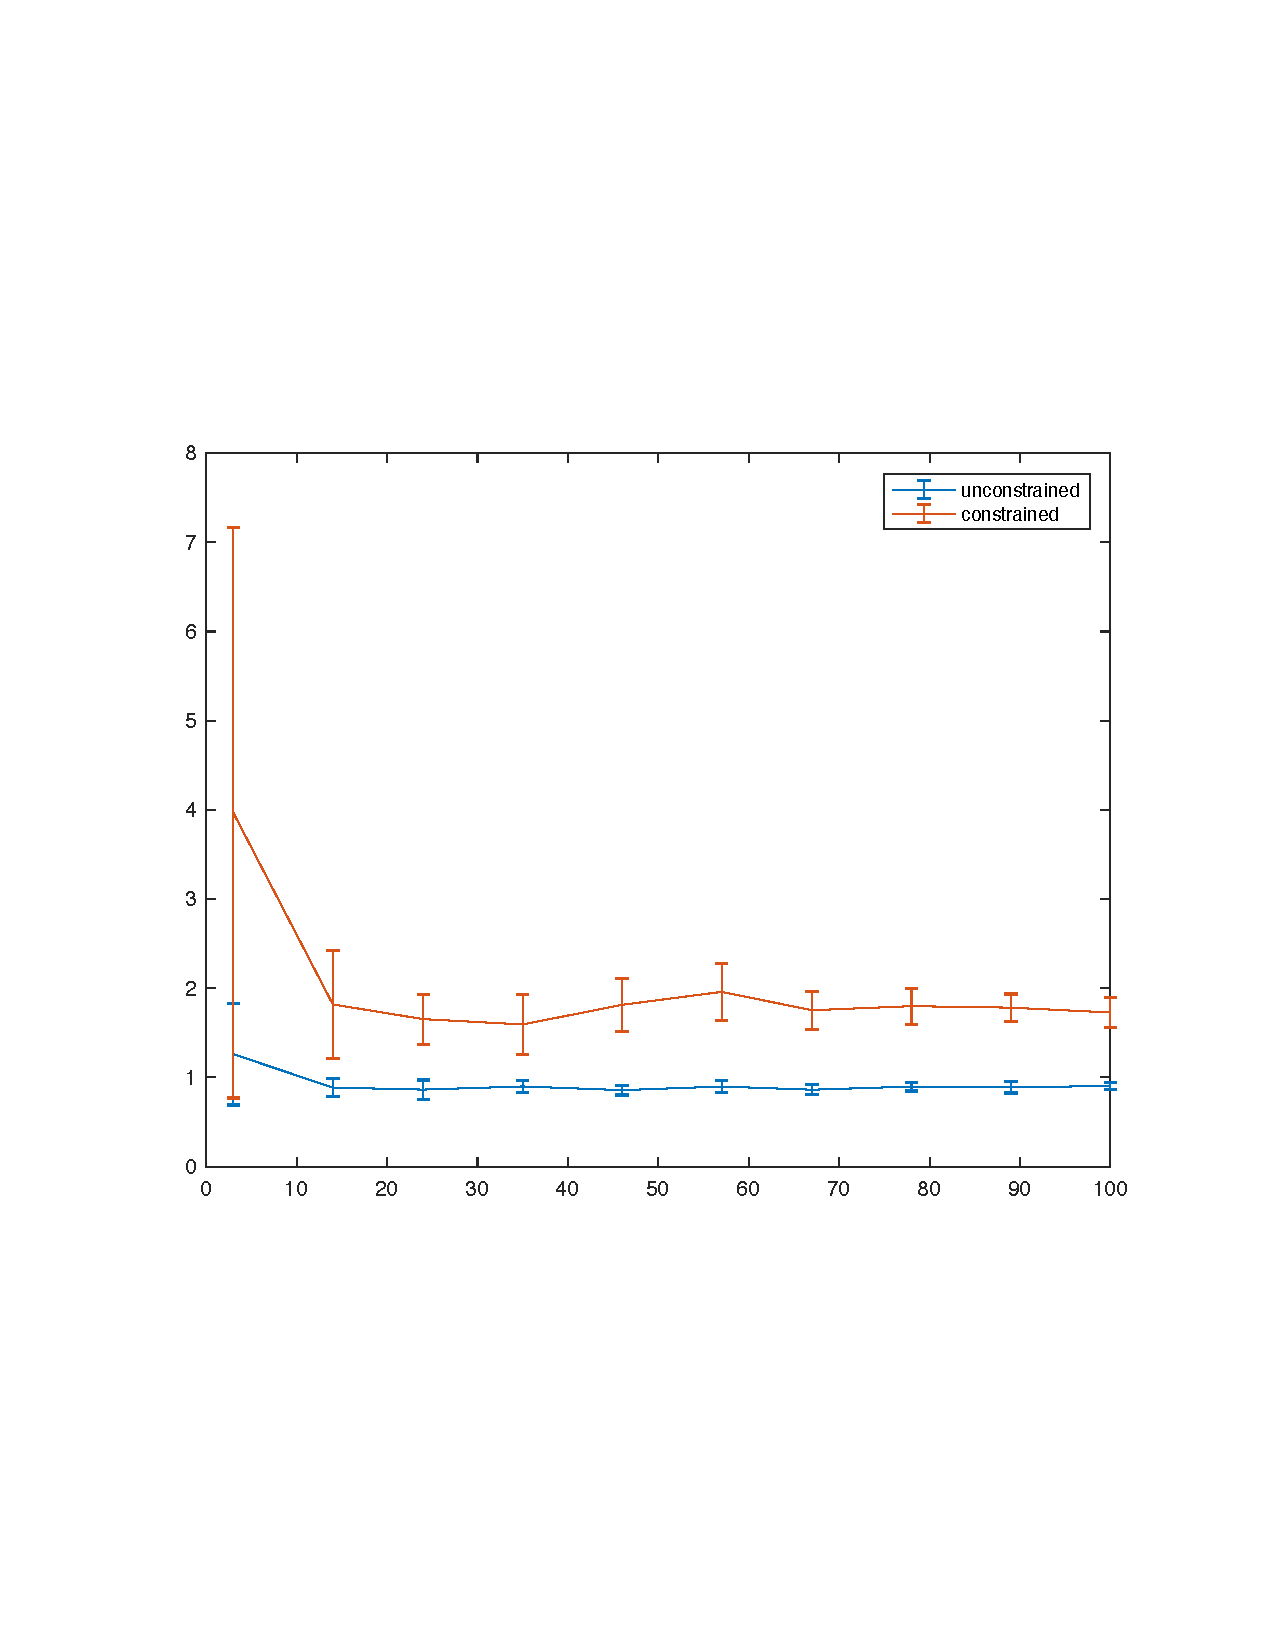
\includegraphics[width=\linewidth]{figure05bound.pdf}
    \subcaption{Test data predictions are bounded to the interval $[0,5]$}
    \label{fig:5b}
\end{minipage}
\caption{We set $d = 100$ and set $\theta \sim \textrm{Unif}[0,1]^{d}$. Then draw training data $x \sim N(0,I_{d})$ and test data $z \sim N(0,I_{d})$ but ensure that $z^{T}\theta \in [a,b]$. Here $n = \sqrt{d}$ and the size of the test set increases along the $x$-axis and the $y$-axis measures error on the test set.}\label{mainfig}
\end{wrapfigure}

Intuitively, incorporating this information should be helpful, however as seen in Figure (\ref{mainfig}), this is not always the case. This write-up elucidates why there can be cases when incorporating this information can in fact be harmful (however for very stupid reasons). For some norm $\lvert \lvert \cdot \lvert \lvert $ let $\theta^{*}_{u}$ denote the optimal variable to the following unconstrained problem,
\begin{equation}
\label{original} 
\begin{aligned}
& \underset{\theta}{\text{minimize}}
& & \sum \limits_{i=1}^{n} \lvert \lvert y_{i} - \theta^{T}x_{i} \lvert \lvert \\
\end{aligned}
\end{equation}

and let  $\theta^{*}_{c}$ denote the optimal variable to the following constrained problem that incorporates our knowledge about the test set,

\begin{equation}
\label{original} 
\begin{aligned}
& \underset{\theta}{\text{minimize}}
& & \sum \limits_{i=1}^{n} \lvert \lvert y_{i} - \theta^{T}x_{i} \lvert \lvert \\
& \text{subject to}
& & \theta^{T}z_{i} \in [a,b], \forall i = 1, \cdots, m.\\
\end{aligned}
\end{equation}
 
 We want to understand when 
 \begin{equation*}
 \sum \limits_{i=1}^{m} \lvert \lvert \theta_{c}^{*T}z_{i} - \theta_{true}^{T}z \lvert \lvert < \sum \limits_{i=1}^{m} \lvert \lvert \theta_{u}^{*T}z_{i} - \theta_{true}^{T}z \lvert \lvert,
 \end{equation*} 
 and visa-versa. 

Let $\{\tilde{x}_{1}, \cdots, \tilde{x}_{k}\}$ be an orthogonal spanning set of $\{x_{1}, \cdots, x_{n} \}$ with corresponding observations $\{\tilde{y}_{1}, \cdots, \tilde{y}_{k} \}$, (i.e. $\tilde{y}_{i} = \theta^{T}\tilde{x}_{i}$ which we can compute from our observations). Extend this set to span the test set so we have $\{ \{\tilde{x}_{1}, \cdots, \tilde{x}_{k}, \tilde{z}_{k+1}, \cdots, \tilde{z}_{k+ \ell}\}$. Let $M$ be the matrix with rows $\tilde{x}_{1}^{T}, \cdots, \tilde{z}_{k+ \ell}^{T}$ so that $M\tilde{x}_{j} = e_{j}$. Then we have for $z_{i}$, $\exists \beta^{(i)}_{j}$ such that,

\begin{equation*}
z_{i} = \sum \limits_{i=1}^{k} \beta_{j}^{(1)} \tilde{x}_{j} + \sum \limits_{i=k+1}^{k + \ell} \beta_{j}^{(1)} \tilde{z}_{j}.
\end{equation*}
Thus 

\begin{align*}
\theta^{T} z_{i} = & \sum \limits_{i=1}^{k} \beta_{j}^{(1)} \theta^{T} \tilde{x}_{j} + \sum \limits_{i=k+1}^{k + \ell} \beta_{j}^{(1)}  \theta^{T} \tilde{z}_{j}  = \sum \limits_{i=1}^{k} \beta_{j}^{(1)} \tilde{y_{j}} + \sum \limits_{i=k+1}^{k + \ell} \beta_{j}^{(1)}  (M\theta^{T})M \tilde{z}_{j} \\
& = \sum \limits_{i=1}^{k} \beta_{j}^{(1)} \tilde{y_{j}} + \sum \limits_{i=k+1}^{k + \ell} \beta_{j}^{(1)}  (M\theta^{T})e_{j} = \sum \limits_{i=1}^{k} \beta_{j}^{(1)} \tilde{y}_{j} + \sum \limits_{i=k+1}^{k + \ell} \beta_{j}^{(1)}  \tilde{\theta}_{j},
\end{align*}
where $\tilde{\theta} = M\theta$. Then 
\begin{align*}
a \leq \theta^{T}z_{i} \leq b \iff  a- \sum \limits_{i=1}^{k} \beta_{j}^{(1)} \tilde{y}_{j}  \leq \sum \limits_{i=k+1}^{k + \ell} \beta_{j}^{(1)}  \tilde{\theta}_{j} \leq b -  \sum \limits_{i=1}^{k} \beta_{j}^{(1)} \tilde{y}_{j}.
\end{align*}
Let $a_{i} = a- \sum \limits_{i=1}^{k} \beta_{j}^{(1)} \tilde{y}_{j} $, $b_{i} = b -  \sum \limits_{i=1}^{k} \beta_{j}^{(1)} \tilde{y}_{j}$,  $\overline{\theta} = \tilde{\theta}_{k+1:k+\ell}$, and $\overline{\beta} = \tilde{\beta}_{k+1:k+\ell}$ so that we have $\forall i$
\begin{equation}
a_{i} \leq \overline{\beta}^{(i)T} \overline{\theta} \leq b_{i}.
\end{equation}
So our optimization problems become 
\begin{enumerate}
\item In the case of the unconstrained case $\theta^{*}_{u} = M^{T}\tilde{\theta}^{*}_{u}$ where $(\tilde{\theta}^{^{*}}_{u})_{j}= \tilde{y}_{j}$ for $j = 1, \cdots, k$ and $(\tilde{\theta}^{^{*}}_{u})_{j}$ can be anything for $j = k+1, \cdots, k+ \ell$. CVX will set these $(\tilde{\theta}^{^{*}}_{u})_{j} = 0$ by default. \\
\item In the case of the constrained case $\theta^{*}_{c} = M^{T}\tilde{\theta}^{*}_{c}$, where again $(\tilde{\theta}^{^{*}}_{c})_{j}= \tilde{y}_{j}$ for $j = 1, \cdots, k$. Suppose we have so few test samples that $\exists \overline{\theta}$ such that $\overline{\beta}_{i}^{T} \overline{\theta} = \frac{1}{2}(b_{i} + a_{i})$ for each $i$. If this is possible, then CVX will return $(\tilde{\theta}^{^{*}}_{u})_{j}  = \frac{1}{2}(b_{i} + a_{i})$. Note that $\frac{1}{2}(b_{i} + a_{i}) = a_{i} + \frac{1}{2}(b_{i} - a_{i} =  a- \sum \limits_{i=1}^{k} \beta_{j}^{(1)} \tilde{y}_{j} + frac{1}{2}(b-a)$.
\end{enumerate}
In the case with few test samples we get that the error for the unconstrained case is 
\begin{align*}
\sum \limits_{i=1}^{m} \lvert \lvert \theta_{u}^{*T}z_{i} - \theta_{true}^{T}z_{i} \lvert \lvert = \sum \limits_{i=1}^{m} \lvert \lvert \overline{\beta}^{(i)T} (\theta_{true})_{k+1:k+\ell} \lvert \lvert ,
\end{align*}
while the error for the constrained case is 
\begin{align*}
\sum \limits_{i=1}^{m} \lvert \lvert \theta_{c}^{*T}z_{i} - \theta_{true}^{T}z_{i} \lvert \lvert = \sum \limits_{i=1}^{m} \lvert \lvert \frac{a+b}{2} - \overline{\beta}^{(i)T} (\theta_{true})_{k+1:k+\ell} \lvert \lvert .
\end{align*}
So we see that if the response of $z$, subtracting out the components that are predictable from the training data, is closer to the origin than it is to the midpoint of the interval (on average), then we are actually better off not incorporating this constraint. 
  \end{document}